\documentclass{standalone}
\usepackage{tikz}
\usetikzlibrary{positioning}

\begin{document}
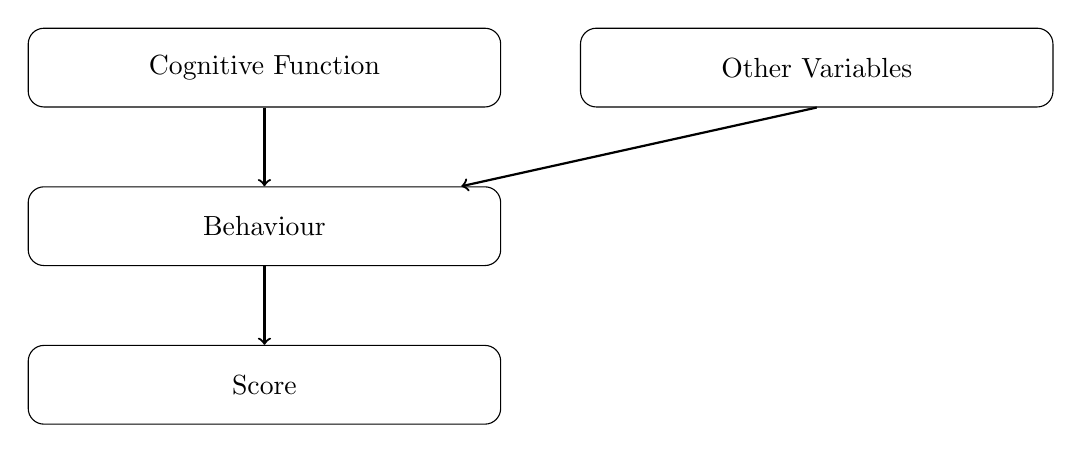
\begin{tikzpicture}[
  node distance=10mm,
  block/.style={
    draw,
    rounded corners=2mm,
    minimum width=6cm,
    minimum height=1cm,
    align=center
  }
]

% Nodes
\node[block] (A) {Cognitive Function};
\node[block, below=of A] (B) {Behaviour};
\node[block, below=of B] (C) {Score};
\node[block, right=of A] (D) {Other Variables};

% Solid connection line from A to B (no arrow)
\draw[->, thick] (A.south) -- (B.north);
\draw[->, thick] (B.south) -- (C.north);
\draw[->, thick] (D.south) -- ([xshift=25mm]B.north);

\end{tikzpicture}
\end{document}
